% chapter4.tex
% Capitulo 4. Resultados
%==========================================================================
\chapter{Resultados}

En este cap\'itulo se muestran los resultados del estudio de la plataforma USRP. El experimento
consisti\'o en transmitir datos generados de una fuente aleatoria por software y de una fuente fija
que consiste en una imagen entre las tarjetas LFTX y LFRX por medio de un cable coaxial. Estos
datos son modulados con el esquema DQPSK como esta implementado en \gnuradio. Despu\'es se
observaron los resultados utilizando las herramientas proporcionadas por \gnuradio y el lenguaje Python.

%Material utilizado
%==========================================================================
\section{Material utilizado}
El material que se utiliz\'o para realizar el experimento fue el siguiente:

\begin{itemize}
  \item 1 USRP
  \item Tarjetas LFTX y LFRX
  \item Cable coaxial con terminales SMA a SMA
  \item Cable USB
  \item Computadora laptop con las siguientes caracter\'isticas:
  \begin {itemize}
    \item CPU Intel Core 2 Duo T5550 a 1.83Ghz
    \item 4GB memoria DDR2
    \item Sistema operativo Ubuntu 10.01
  \end{itemize}
\end{itemize}

Los programas \verb|benchmark_tx.py| y \verb|benchmark_rx.py| de la carpeta de ejemplos del codigo
fuente fueron utilizados para realizar la transmisi\'on, ya que estos ejemplos son programas
completos y maduros que ayudan a ilustrar varias caracter\'isticas de la programaci\'on con
\gnuradio. Los programas \verb|benckmark_tx2.py| y \verb|benchmark_rx2.py| tienen la misma
estructura que su versi\'on anterior pero estos implementan el modulador y demodulador utilizando la
t\'ecnica de filtros polif\'asicos. Esta versi\'on, incluyendo los bloques que implementan estos
filtros, fueron incluidos en el c\'odigo fuente el 23 de Marzo de 2010 y fueron incluidos en este
estudio para comparar el rendimiento de ambas versiones.


%Parametros utilizados
%==========================================================================
\section{Par\'ametros utilizados}

Para ejecutar los ejemplos \verb|benchmark_tx.py| y \verb|benchmark_rx.py| es neceario moverse al
directorio donde se encuentran. La ruta es:
\begin{center}
\verb|<dir_donde_esta_el_codigo_fuente>|/\verb|gnuradio-examples|/\verb|python|/\verb|digital|
\end{center}
Los programas se ejecutan por medio de la consola de texto utilizando la notacion \verb|./| para
indicar que se va correr un ejecutable. La sintaxis completa es:
\begin{center}
\verb|./benchmark_tx.py <opciones>|
\end{center}
donde opciones son algunas opciones que se pueden pasar al programa para controlar su
funcionamiento. Para ver todas las opciones que soporta se puede utilizar el siguiente comando:
\begin{center}
\verb|./benchmark_tx.py --help|
\end{center}

Los opciones que se utilizaron para el transmisor y receptor son los siguientes:

\section*{TRANSMISOR}
\begin{itemize}
  \item \textbf{-m}: Especifica el modulador que se va utilizar. La opci\'on que se utilizo fue
  DQPSK y DBPSK. BPSK se utilizo para realizar la comparaci\'on entre ambos esquemas.
  \item \textbf{-r}: Especifica la taza de bits. Se utilizaron varios valores desde 100kbps hasta
  10kbps. Este valor depende mucho de la PC que se est\'e utilizando ya que valores muy altos
  dependen del rendimiento del CPU.
  \item \textbf{--tx-amplitude}: Especifica la amplitud de la se\~nal generada por el DAC en el
  USRP. Sus valores van de 0 a 1. Se utilizo el valor default de 0.25.
  \item \textbf{--excess-bw}: Especifica el par\'ametro $\beta$ del filtro acoplador de coseno
  elevado. Su rango de valores es de 0 a 1. Se utilizaron tres valores para el an\'alisis: 0.35,
  0.50 y 0.75.
  \item \textbf{-f}: Especifica la frecuencia con la cual se van a sintonizar las tarjetas
  auxiliares. Para este estudio se estuvo utilizando la frecuencia m\'axima que soportan las
  tarjetas LFTX y LFRX que es 30Mhz.
  \item \textbf{-S}: Especifica la cantidad de muestras por s\'imbolo. El valor default es de 2. Se
  observo que se tuvo un mejor rendimiento con un valor de 4.
\end{itemize}

\section*{RECEPTOR}
\begin{itemize}
  \item \textbf{-m}: Especifica el demodulador que se va utilizar. Igual que en el transmisor se
  utiliz\'o DQPSK y DBPSK.
  \item \textbf{--gain-mu}: Especifica la ganancia que se utiliza en el lazo de costas para la
  detecci\'on de la fase. Se utilizo un valor de 0.5.
  \item \textbf{-f}: Especifica la frecuencia a la que se sintoniza la tarjeta RX. Se utiliz\'o un
  valor de 30Mhz.
  \item \textbf{-S}: Especifica la cantidad de muestras por s\'imbolo utilizada en el demodulador.
  Igual que en el transmisor se utilizo un valor de 4.
  \item \textbf{-r}: Especifica la taza de bits. Se utilizaron los mismos valores que en el
  transmisor.
  \item \textbf{--excess-bw}: Especifica el par\'ametro $\beta$ del filtro acoplador de coseno
  elevado. Se utilizaron los mismos valores que en el transmisor.
\end{itemize}

Cabe mencionar que debido a que los dos programas son independientes uno del otro, es necesario
igualar algunos par\'ametros para lograr una transmisi\'on exitosa. Los par\'ametros \verb|--f|,
\verb|-S|, \verb|-r| y \verb|--excess-bw| son un ejemplo de estos parametr\'os. Todos los
par\'ametros tienen valores default si no se desea modificarlos pero uno de ellos es obligatorio
especificarlo y es el de la frecuencia de sintonizaci\'on \verb|-f|. Si se ejecutan los programas
sin especificar este par\'ametro, aunque se especifiquen los otros, marcara un error pidiendo que
se especifique la frecuencia de operacion. 
%Taza de error de bits
%==========================================================================
\section{Taza de error de bits}

%TODO: Realizar diagrama de los grafos que se desarrollaron e incluir las graficas del ber.
El an\'alisis de la tasa de error de bits (Bit error rate o BER por sus siglas en ingles) se realizo
para ambos modelos de DQPSK proporcionados por \emph{GNURadio}. El programa que se utilizo fue
basado en un estudio generado y publicado en la pagina de \gnuradio sobre una versi\'on mas optima
del modulador GMSK. El programa fue modificado para que pudiera analizar y comparar ambos esquemas
DBPSK y DQPSK en sus dos versiones: costas/MM y filtros polifasicos.

La estructura del programa est\'a dividida en 3 etapas. La primera etapa genera una se\~nal de una
fuente de n\'umeros pseudo-aleatorios y luego la modula utilizando el modulador que se va a evaluar.
Los datos arrojados del modulador son enviados a archivos que se utilizaran como la entrada para las
siguientes etapas. El programa define una clase llamada \verb|SigGen| derivada de la clase
\verb|top_block| para definir un grafo de flujo de datos. La estructura del grafo se muestra en la
figura \ref{fig:siggen}.

\begin{figure}[htp]
  \centering
  \vspace{0.3in}
  \begin{tikzpicture}[scale=0.8, transform shape, node distance=0.5cm and 0.4cm]
  	\node (glfsr) [grblock] {\footnotesize{Fuente de n\'umeros pseudo-aleatorios}};
  	\node (limiter) [grblock, right=of glfsr] {\footnotesize{Limitador de datos}}
  	edge [<-] (glfsr);
  	\node (srcbits) [grblock, below=of limiter] {\footnotesize{src\_bits.dat}}
  	edge [<-] (limiter);
  	\node (unpacktopack) [grblock, right=of limiter] {\footnotesize{Empaquetado de bits}}
  	edge [<-] (limiter);
  	\node (newmod) [grblock, above right=of unpacktopack] {\footnotesize{Mod\_Demod \\ Poly}};
  	\draw [->] (unpacktopack.east) -- ++(0.2,0) |- (newmod);
  	\node (cleanbb) [grblock, right=of newmod] {\footnotesize{limpio\_bb.dat}}
  	edge [<-] (newmod);
  	\node (oldmod) [grblock, below right=of unpacktopack] {\footnotesize{Mod\_Demod \\ Costas\_MM}};
  	\draw [->] (unpacktopack.east) -- ++(0.2,0) |- (oldmod);
  	\node (cleanoldbb) [grblock, right=of oldmod] {\footnotesize{limpio\_oldbb.dat}}
  	edge [<-] (oldmod);
  \end{tikzpicture}
  \vspace{0.3in}
  \caption{Grafo generador de datos modulados para la evaluaci\'on del BER.}
  \label{fig:siggen}
\end{figure}

Los bloques se describen de la siguiente manera:

\begin{itemize}
  \item \textbf{Fuente de n\'umeros pseudo-aleatorios}: El bloque se genera por medio de la clase
  \verb|gr.glfsr_source_b|. Esta clase implementa un registro de desplazamiento con
  retroalimentaci\'on lineal en modo Galois. El sufijo ``b'' indica que el generador entrega valores
  binarios. El par\'ametro que se le especifica es el numero de bits de precisi\'on para generar
  una secuencia de bits de longitud $2^{N-1}$, el cual expresa la m\'axima cantidad de valores
  que puede generar antes de ciclarse \cite{xilinx}. 
  \item \textbf{Limitador de datos}: Este bloque se genera por medio de la clase \verb|gr_head|, el
  cual su funci\'on es tomar una cierta cantidad de valores en su entrada y descartar todo lo
  dem\'as. A esta secuencia de valores se le anexa el valor especial \emph{EOF} que especifica el
  fin del flujo dentro del grafo. Esto causar\'a que el grafo termine su ejecuci\'on una vez que
  este valor se propague a todos los bloques. Sus par\'ametros el tipo de datos con el que va
  trabajar y la cantidad de muestras que va dejar pasar de su entrada a su salida.
  \item \textbf{Source\_bits.dat, Limpio\_bb.dat, Limpio\_oldbb.dat}: Estos bloques utilizan la
  clase \verb|gr.file_sink| para enviar el flujo de datos a un archivo. En este grafo se generan tres
  archivos para guardar los bits originales y los bits modulados con los dos tipos de moduladores
  de \emph{GNURadio}. Sus par\'ametros son el tipo de datos que van a escribir y el nombre del
  archivo.
  \item \textbf{Empaquetado de bits}: Este bloque se implementa utilizando la clase \\
  \verb|gr.unpacked_to_packed_bb|. Se encarga en juntar los bits que entrar y formar bytes completos
  en la salida. Estos bytes representan la informaci\'on original.
  \item \textbf{Mod\_Demod Poly y Mod\_Demod Costas\_MM}: Estos bloques representan los moduladores
  que se evaluaron durante el experimento y se implementan con las clases \verb|blks2.dqpsk_mod| y
  \verb|blks2.dqpsk2_mod| respectivamente.
\end{itemize}

El c\'odigo que implementa este grafo se muestra en el listado \ref{ex:siggen}.

\begin{lstlisting}[float, label=ex:siggen, caption={C\'odigo que implementa el grafo
generador de se\~nales.}, breaklines=true]
class SigGen(gr.top_block):
  def __init__(self,num_bits=5000,pn_degree=23,xmit_bt=0.25,samp_per_symbol=8):
    gr.top_block.__init__(self, 'SigGen')
	
	src = gr.glfsr_source_b(pn_degree)
	src_limiter = gr.head(gr.sizeof_char, num_bits)

    bit_packer = gr.unpacked_to_packed_bb(1, gr.GR_MSB_FIRST)
    mod = blks2.dqpsk2_mod(samp_per_symbol, xmit_bt)

    bit_packer_old = gr.unpacked_to_packed_bb(1, gr.GR_MSB_FIRST)
    mod_old = blks2.dqpsk_mod(samp_per_symbol, xmit_bt)

    self.connect(src, src_limiter)
    self.connect(src_limiter, gr.file_sink(gr.sizeof_char, 'src_bits.dat'))
    self.connect(src_limiter, bit_packer, mod, gr.file_sink(gr.sizeof_gr_complex, 'limpio_bb.dat'))
    self.connect(src_limiter, bit_packer_old, mod_old, gr.file_sink(gr.sizeof_gr_complex, 'limpio_old_bb.dat'))
\end{lstlisting}

La segunda etapa toma la se\~nal modulada de los archivos y los pasa a trav\'es de un grafo que
aplica ruido Gaussiano para simular un canal de transmisi\'on AWGN. El grafo se muestra en la figura
\ref{fig:noisegen}.

\begin{figure}[htp]
  \centering
  \vspace{0.3in}
  \begin{tikzpicture}[scale=0.8, transform shape, node distance=15mm and 20mm]
  	\node (sigsource) [grblock] {\footnotesize{Fuente de datos de un archivo}};
  	\node (noisesource) [grblock, below=of sigsource] {\footnotesize{Fuente de ruido}};
  	\node (sum) [op, below right=of sigsource, yshift=1.4cm] {$\sum$};
  	\draw [->] (sigsource.east) -- ++(1,0) |- (sum);
  	\draw [->] (noisesource.east) -- ++(1,0) |- (sum);
  	\node (noisesig) [grblock, right=of sum] {\footnotesize{Archivo \\ ruido\_bb.dat}}
  	edge [<-] (sum);
  	\node (noisedat) [grblock, below=of noisesource] {\footnotesize{Archivo ruido.dat}}
  	edge [<-] (noisesource);
  \end{tikzpicture}
  \vspace{0.3in}
  \caption{Grafo que simula un canal AWGN}
  \label{fig:noisegen}
\end{figure}

El grafo toma como entrada caracter\'istica el valor de la relaci\'on de energ\'ia de bit a ruido
$E_b/N_0$ que se va utilizar en el an\'alisis. Los bloques se implementan de la siguiente manera:

\begin{itemize}
  \item \textbf{Fuente de datos de archivo}: Este bloque se implementa con la clase
  \verb|gr.file_source|. Se utiliza para leer el archivo generado del grafo \ref{fig:siggen} que
  contiene los bits modulados.
  \item \textbf{Fuente de ruido}: Este bloque se implementa usando la clase \\
  \verb|gr.noise_source_c|. El prefijo ``c'' indica que trabaja con datos complejos. La clase acepta
  dos par\'ametros de entrada: el tipo de ruido que se quiere generar y la magnitud. El tipo de
  ruido puede ser una de las siguientes constantes:
  \begin{itemize}
    \item \verb|GR_UNIFORM|
    \item \verb|GR_GAUSSIAN|
    \item \verb|GR_LAPLACIAN|
    \item \verb|GR_IMPULSE| 
  \end{itemize}
  Para simular el canal AWGN se utiliz\'o la constante \verb|GR_GAUSSIAN|.
  \item \textbf{Archivo ruido\_bb.dat y Archivo ruido.dat}: Este bloque usa la clase
  \verb|file_sink_c| para guardar los datos complejos que representan la se\~nal mezclada con el
  ruido. El archivo ruido.dat guarda los datos que representan el puro ruido sin la se\~nal
  modulada.
\end{itemize}

Para determinar la magnitud del ruido el programa primero calcula la potencia promedio del archivo
que contiene la se\~nal modulada sin ruido, la energ\'ia por bit y por \'ultimo la magnitud del
ruido. La potencia se calcula utilizando la siguiente expresi\'on:

\begin{equation}\label{eq:bitpower}
P_{prom}=\frac{1}{N}\sum_{n=1}^{N}{x^2(n)}
\end{equation}

La energ\'ia por bit se calcula a partir de la potencia como se muestra en la siguiente
expresi\'on:

\begin{equation}\label{eq:bitenergy}
E_b=\frac{P_{prom}}{f_b}
\end{equation}
donde $f_b$ es la taza de bits en bits por segundo.

El listado \ref{ex:powenerprogram} muestra dos funciones en Python que calculan estos dos
par\'ametros.

\begin{lstlisting}[float, label=ex:powenerprogram, caption={Funciones en Python para calcular la
potencia y la energia promedio de una se\~nal}]
def get_p_avg_watts(fn, is_complex=False):

    f = open(fn)
    d = f.read()
    num_floats = (len(d)/4)
    d = struct.unpack('f'*num_floats, d)
    if is_complex:
        d = d[::2] #toma la parte real
    d_sq = [x*x for x in d]
    return sum(d_sq)/len(d_sq)
    
def get_eb_joules(fn, bits_per_sec, is_complex=False):

    p_avg = get_p_avg_watts(fn, is_complex=is_complex)
    return p_avg / bits_per_sec

\end{lstlisting}

El c\'odigo que implementa el grafo \ref{fig:noisegen} se muestra en el listado \ref{ex:pynoisegen}.

\begin{lstlisting}[float, label=ex:pynoisegen, caption={C\'odigo que implementa el grafo generador
de ruido}, breaklines=true]

class NoiseGen(gr.top_block):
  def __init__(self, ebn0_dB, bits_per_sec, samp_per_sec):
    gr.top_block.__init__(self, 'NoiseGen')

    ebn0_ratio = dB_to_ratio(ebn0_dB)

    n0_watts_per_Hz = bertool.get_eb_joules(fn = 'limpio_bb.dat', bits_per_sec = bits_per_sec) / ebn0_ratio 
    n_mag = sqrt(0.5 * n0_watts_per_Hz * samp_per_sec)
    n_src = gr.noise_source_c(gr.GR_GAUSSIAN, n_mag)
    sig_src = gr.file_source(gr.sizeof_gr_complex, 'limpio_bb.dat')
    adder = gr.add_cc()

    self.connect(sig_src, adder, gr.file_sink(gr.sizeof_gr_complex, 'ruido_bb.dat'))
    self.connect(n_src, (adder, 1))
    self.connect(n_src, gr.file_sink(gr.sizeof_gr_complex, 'ruido.dat'))
\end{lstlisting}

La tercera etapa realiza la demodulaci\'on de las se\~nales capturadas por los grafos anteriores.
Esta etapa consiste en leer la se\~nal mezclada con ruido, aplicar un filtro pasa bajas pre-selector
para seleccionar la porci\'on del canal que nos interesa, demodular la se\~nal recibida y guardar los
datos generados en un archivo para realizar la comparaci\'on. La estructura del grafo que realiza esta
etapa se muestra en la figura \ref{fig:analizer}.

\begin{figure}[htp]
  \centering
  \vspace{0.3in}
  \begin{tikzpicture}[scale=0.8, transform shape]
  	\node (sigsource) [grblock] {\footnotesize{Archivo con se\~nal y ruido}};
  	\node (fir) [grblock, right=of sigsource] {\footnotesize{Filtro pre-selector}}
  	edge [<-] (sigsource);
  	\node (demod) [grblock, right=of fir] {\footnotesize{Demodulador}}
  	edge [<-] (fir);
  	\node (sink) [grblock, below=of demod] {\footnotesize{bits\_demod\_bb.dat}}
  	edge [<-] (demod);
  \end{tikzpicture}
  \vspace{0.3in}
  \label{fig:analizer}
  \caption{Grafo que realiza la demodulaci\'on de la se\~nal simulada}
\end{figure}

El grafo tiene un par\'ametro obligatorio y es el demodulador que se va utilizar para el an\'alisis.
Los dem\'as son opcionales y establecen los par\'ametros de muestras por s\'imbolos, s\'imbolos
por segundo y los par\'ametros de ancho de banda para el filtro pre-selector. Para este an\'alisis
se utilizaron los valores por default. Los resultados del filtro se muestran en la figura
\ref{fig:predetect}.

\begin{figure}[htp]
  \centering
  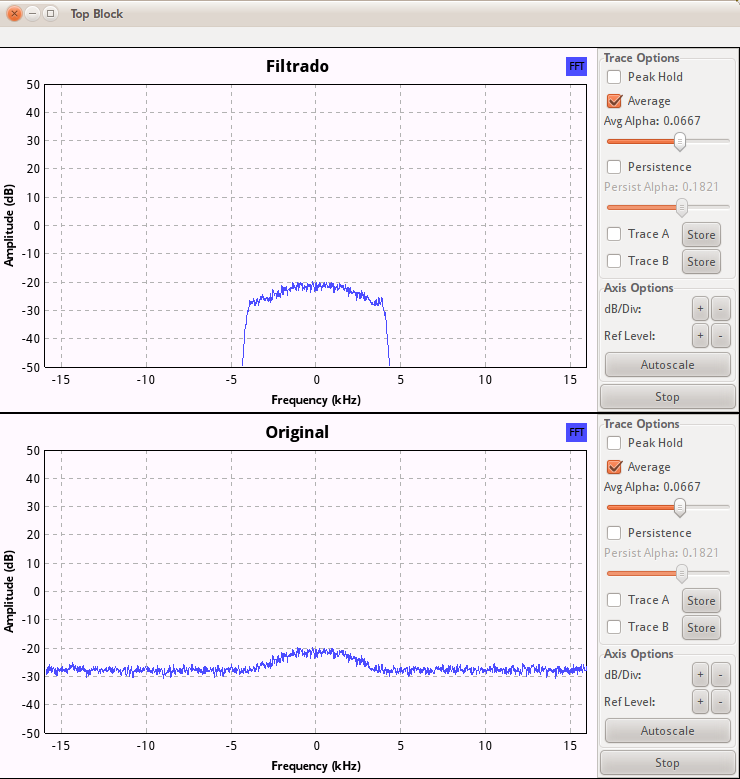
\includegraphics[scale=0.5]{figs/predetectfilter}
  \caption{Respuesta del filtro pre-selector en el receptor para la medici\'on del BER.}
  \label{fig:predetect}
\end{figure}

Los bloques del grafo se implementan de la siguiente manera:

\begin{itemize}
  \item \textbf{Archivo con se\~nal y ruido}: La clase \verb|gr.file_source_c| se encarga de leer el
  archivo generado por el grafo \verb|NoiseGen| para enviarlo al filtro pre-selector.
  \item \textbf{Filtro pre-selector}: El filtro pasa bajas se implementa con una combinacion de dos
  clases: \verb|gr.firdes.low_pass| y \verb|gr.fir_filter_ccf|. El primero se utiliza para generar
  los coeficientes del filtro a partir de los par\'ametros de entrada que se le especifiquen. Se
  utilizaron los valores default del ejemplo a excepci\'on de la ventana. Originalmente utilizaba
  una ventana de tipo Hamming y se cambio a una ventana Kaizer ya que esta tuvo mejor rendimiento y
  ayudo a generar una curva de BER m\'as suave. Los par\'ametros que acepta la clase son la
  ganancia, la frecuencia de muestreo, la frecuencia de corte, el ancho de la banda de transici\'on
  y el tipo de ventana. La segunda clase implementa en si el filtro fir a partir de los coeficientes
  generados por la clase \verb|gr.firdes.low_pass|. Sus par\'ametros de entrada son el factor de
  decimaci\'on y los coeficientes del filtro.
  \item \textbf{Demodulador}: Este bloque representa el demodulador que se est\'a evaluando. En este
  caso fueron ambos DQPSK y DBPSK en sus dos versiones. Las clases que los implementan se encuentran
  dentro del paquete \verb|blks2|. Su uso se muestra en el listado \ref{ex:mainber}. La clase toma
  la se\~nal filtrada e inicia el proceso de demodulaci\'on y detecci\'on. Los resultados son una serie de bits
  desempaquetados, osea, bits individuales.
  \item \textbf{Archivo bits\_demod\_bb.dat}: Este bloque usa la clase \verb|gr.file_sink| para
  escribir a un archivo los bits resultantes del bloque demodulador.
\end{itemize}

El codigo que implementa el tercer grafo se muestra en el listado.

\begin{lstlisting}[float, label=ex:analizer, caption={C\'odigo que implementa el grafo demodulador
para el analisis del BER.}, breaklines=true]
class Analyser(gr.top_block):
    def __init__(self, bb_src_fn, test_demod, samp_per_sym = 8,
                 sym_per_sec = 1e6, pre_detect_filt_bt = 0.9, filt_transition_ratio = 0.1):
        gr.top_block.__init__(self, 'Analyser')

        self.bb_src_fn = bb_src_fn
        self.samp_per_sym = samp_per_sym
        samp_per_sec = samp_per_sym * sym_per_sec

        bb_src = gr.file_source(gr.sizeof_gr_complex, bb_src_fn)

        pre_detect_filt_bw = sym_per_sec * pre_detect_filt_bt
        pre_detect_filt_taps = gr.firdes.low_pass(1.0, samp_per_sec,
                pre_detect_filt_bw, filt_transition_ratio * samp_per_sec,
                gr.firdes.WIN_KAISER, 4.5)
        pre_detect_filt = gr.fir_filter_ccf(1, pre_detect_filt_taps)
        self.connect(bb_src, pre_detect_filt, test_demod)

        self.test_demod_dst_fn = 'bits_demod_bb.dat'
        self.dst = gr.file_sink(gr.sizeof_char, self.test_demod_dst_fn)
        self.connect(test_demod, self.dst)
\end{lstlisting}

El programa principal inicializa los tres grafos y realiza una serie de pruebas para generar la
grafica del BER. La metodolog\'ia que se sigui\'o fue generar varios valores de $E_b/N_0$, desde
12db hasta 2db en intervalos de 0.5db y ejecutar los tres grafos para generar los resultados. Estos
resultados se van guardando en un arreglo y posteriormente se grafican. Los par\'ametros que se
utilizaron para la simulaci\'on fueron los siguientes:

\begin{itemize}
  \item \textbf{Numero de bits}: 20000
  \item \textbf{Muestras por s\'imbolo}: 7
  \item \textbf{S\'imbolos por segundo}: $1e6$
  \item \textbf{Exceso de ancho de banda}: 0.75
\end{itemize}

El c\'odigo del programa principal se muestra en el listado \ref{ex:mainber}. El programa original
se modifico para que pueda evaluar ambos esquemas a la vez.

\begin{lstlisting}[float=hp, breaklines=true]
if __name__ == "__main__":
    num_bits = 20000
    samp_per_sym = 7
    sym_per_sec = 1e6
    samp_per_sec = sym_per_sec * samp_per_sym
    print "Samples per second: ", samp_per_sec
    xmit_bt = 0.75
    ebn0s_dB = list(numpy.arange(12.0, 1.999, -0.5))
    recv_bt = 0.9
    recv_filt_transition_ratio = 0.1

    sg = SigGen(num_bits = num_bits, xmit_bt = xmit_bt, samp_per_symbol = samp_per_sym)
    sg.run()
    del sg

    dbpsk2_demod_bers = []
    dqpsk2_demod_bers = []
    dbpsk2_delay = None
    dqpsk2_delay = None

    for ebn0_dB in ebn0s_dB:
        print ebn0_dB
        ng = NoiseGen(ebn0_dB = ebn0_dB, bits_per_sec = sym_per_sec, samp_per_sec = samp_per_sec)
        ng.run()
        del ng

        #========================
        # Analisis de DQPSK
        #========================

        test_dqpsk2_demod = blks2.dqpsk_demod(samples_per_symbol = samp_per_sym, excess_bw = xmit_bt)

        a = Analyser(bb_src_fn = 'noisy_qpsk2_bb.dat', test_demod = test_dqpsk2_demod, samp_per_sym = samp_per_sym,
                     sym_per_sec = sym_per_sec, pre_detect_filt_bt = recv_bt,
                     filt_transition_ratio = recv_filt_transition_ratio)

        a.run()
        a.close()
        del a

        if dqpsk2_delay is None:
            dqpsk2_delay = bertool.get_delay('src_bits.dat', 'test_demod_dst_bits.dat')
        ber_stats = bertool.get_ber_stats('src_bits.dat', 'test_demod_dst_bits.dat', dqpsk2_delay)
        dqpsk2_demod_bers.append(ber_stats[0])
\end{lstlisting}

\begin{lstlisting}[float=hp, label=ex:mainber, caption={C\'odigo Python de la rutina principal del
analisis del BER.}, breaklines=true]
        #========================
        # Analisis de DBPSK
        #========================

        test_dbpsk2_demod = blks2.dbpsk_demod(samples_per_symbol = samp_per_sym, excess_bw = xmit_bt)

        a = Analyser(bb_src_fn = 'noisy_bpsk2_bb.dat', test_demod = test_dbpsk2_demod, samp_per_sym = samp_per_sym,
                     sym_per_sec = sym_per_sec, pre_detect_filt_bt = recv_bt,
                     filt_transition_ratio = recv_filt_transition_ratio)

        a.run()
        a.close()
        del a

        if dbpsk2_delay is None:
            dbpsk2_delay = bertool.get_delay('src_bits.dat', 'test_demod_dst_bits.dat')
        ber_stats = bertool.get_ber_stats('src_bits.dat', 'test_demod_dst_bits.dat', dbpsk2_delay)
        dbpsk2_demod_bers.append(ber_stats[0])


    ebn0s_dB.reverse()
    dbpsk2_demod_bers.reverse()
    dqpsk2_demod_bers.reverse()

    fig = p.figure()
    p.title(u'Desempeño de DQPSK y DBPSK')
    ax = fig.add_subplot(111)
    ax.semilogy(ebn0s_dB, dqpsk2_demod_bers, 'b', label = 'DQPSK')
    ax.hold(True)
    ax.semilogy(ebn0s_dB, dbpsk2_demod_bers, 'r', label = 'DBPSK')
    ax.hold(False)

    ax.yaxis.grid(True, which = 'minor')
    ax.xaxis.grid(True)

    p.legend()

    p.ylabel('BER')
    p.xlabel('Ebn0_dB')
    p.show()
\end{lstlisting}

Los resultados de la primera versi\'on de los esquemas DQPSK y DBPSK se muestran en la figura
\ref{fig:bernormal}.

\begin{figure}[htp]
  \centering
  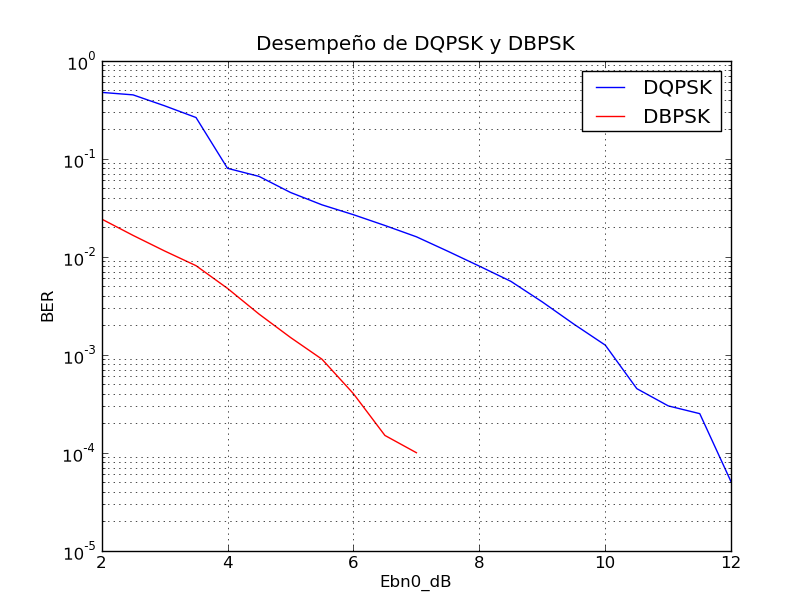
\includegraphics[scale=0.7]{figs/bernormal}
  \caption{Grafica comparativa del BER para la primera versi\'on de los esquemas DQPSK y DBPSK.}
  \label{fig:bernormal}
\end{figure}

Los resultados muestran el rendimiento entre los dos esquemas de modulaci\'on a diferentes niveles
de SNR. Debido a que DQPSK utiliza dos bits por s\'imbolo tiene m\'as probabilidades de generar
errores a niveles muy altos de ruido. Para poder lograr niveles confiables de transmisi\'on se
requiere mas potencia que DBPSK.

La segunda versi\'on de estos esquemas intenta mejorar el BER por medio de la implementaci\'on de
bancos de filtros polif\'asicos. La misma metodolog\'ia se sigui\'o para su an\'alisis y los
resultados se muestran en la figura \ref{fig:berpoly}. Como se puede observar, los filtros
polif\'asicos ofrecen una mejora en el rendimiento de ambos esquemas. A niveles bajos de SNR DQPSK
tiene un poco mas de tolerancia que la versi\'on anterior para generar errores. Con estos se
demuestra el rendimiento del c\'odigo fuente actual de \emph{GNURadio}. 

\begin{figure}[t]
  \centering
  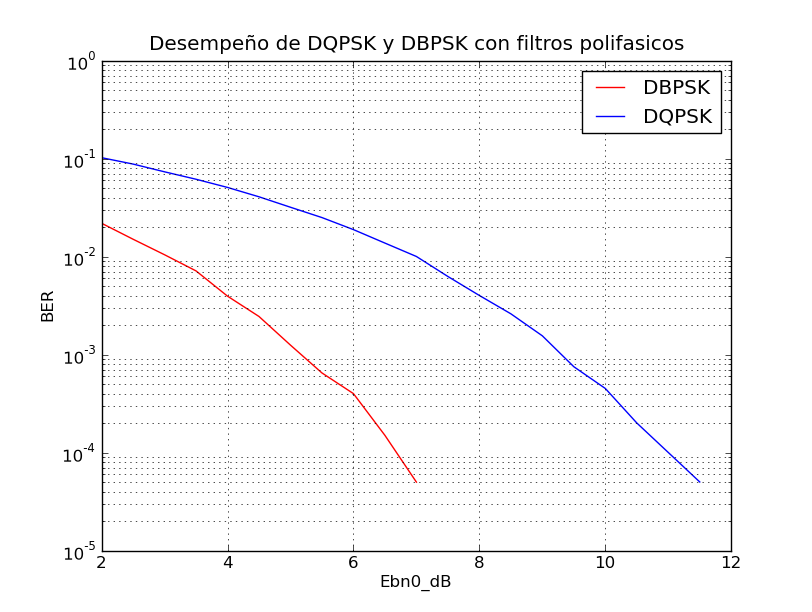
\includegraphics[scale=0.7]{figs/berpoly}
  \caption{Grafica comparativa del BER para la segunda versi\'on de los esquemas DQPSK y DBPSK.}
  \label{fig:berpoly}
\end{figure}

%Espectrograma de la transmision
%==========================================================================
\section{Espectrograma de la transmisi\'on}

\gnuradio contiene varias herramientas para visualizar las se\~nales que se transmiten y se reciben.
Estas herramientas son programas completos que se pueden utilizar como base para elaborar programas
m\'as complejos. Una de estas herramientas visuales es un espectrograma que permite ver la densidad
espectral de potencia de una se\~nal que se est\'a recibiendo. La compilaci\'on del c\'odigo fuente
instala este programa en \verb|/usr/bin/| para que se pueda acceder a ella de manera global. El
programa se llama \verb|usrp_fft.py| y se encuentra originalmente en la carpeta \verb|gr-utils| del
c\'odigo fuente. Este programa se puede acceder desde aqui o bien desde su lugar global por medio de
la consola de comandos. El programa proporciona varios par\'ametros que permiten que se configure de
diferentes maneras dependiendo del uso que se le va dar. Estos par\'ametros son los siguientes:

\begin{itemize}
  \item \textbf{-w}: Selecciona el USRP que se va utilizar en caso de haber mas de uno conectado a
  la PC.
  \item \textbf{-R}: Selecciona el lado RX que se va utilizar en el USRP: Lado A o Lado B. Esto lo
  determina el lugar donde este conectada la tarjeta auxiliar que se va utilizar.
  \item \textbf{-A}: Selecciona la antena que se va utilizar. Esto solo se utiliza con las tarjetas
  de la serie RFX.
  \item \textbf{-d}: Selecciona el valor de decimacion con el que se configurar\'a el DDC del FPGA.
  Por default lo configura a 16.
  \item \textbf{-f}: Especifica la frecuencia con la que se sintoniza la tarjeta auxiliar.
  \item \textbf{-g}: Especifica la ganancia con la que se programa el amplificador programable. Los
  valores son en decibeles.
  \item \textbf{-W}: Activa la opcion de utilizar el espectrograma. Por default la aplicacion actua
  como un analizador de espectros, desplegando la FFT de la se\~nal recibida.
  \item \textbf{-S}: Activa la opcion de utilizar el osciloscopio.
  \item \textbf{--fft-size}: Especifica el tama\~no de muestras que utiliza la FFT. Por default
  utiliza 1024 muestras.
\end{itemize} 

Este programa se utilizo durante la transmisi\'on de los datos generados por los programas
\verb|benchmark_tx.py| y \verb|benchmark_rx.py| para observar la densidad espectral de potencia de
la portadora. Las opciones que se utilizaron para configurar el programa fueron las siguientes:

\begin{center}
\verb|usrp_fft.py -f 30M -d 256 -W|
\end{center}

El espectrograma se muestra en la figura \ref{fig:spectrogramgui}.

\begin{figure}[htp]
  \centering
  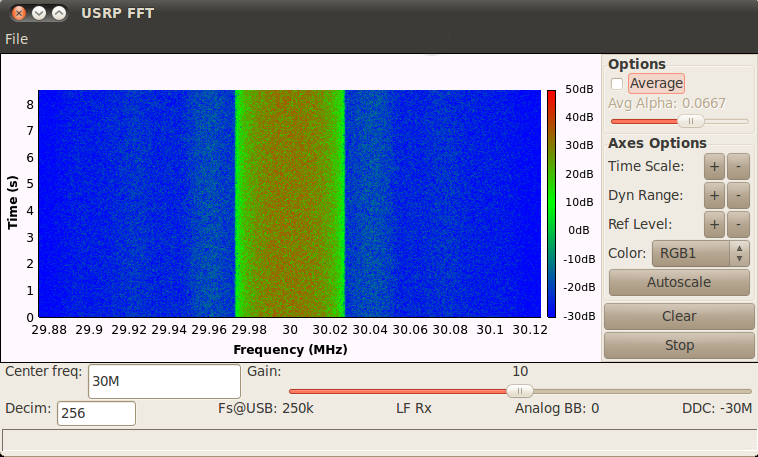
\includegraphics[scale=0.7]{figs/spectrogramgui}
  \caption{Aplicaci\'on en Python que muestra el espectrograma de lo que el USRP esta recibiendo.}
  \label{fig:spectrogramgui}
\end{figure}

El espectrograma consiste en una grafica de cascada (waterfall en ingl\'es) que se despliega en
forma vertical (algunos autores la despliegan en forma horizontal). El eje Y es el tiempo medido en
segundos y la grafica se desplaza de abajo hacia arriba. El eje X representa el espectro en Hz. La
figura \ref{fig:spectrogramgui} muestra la intensidad de la portadora de 30Mhz centrada en la
grafica. Los colores tenues a un lado de la barra verde representan las bandas laterales de la
portadora. Desde esta aplicaci\'on es posible modificar varios par\'ametros del USRP como la
ganancia, la frecuencia y el valor de decimaci\'on del DDC. Los ejes tambi\'en se pueden ajustar por
medio de las opciones que aparecen en la derecha de la pantalla (Time Scale, Dyn Range, Ref Level).
En este ejemplo la portadora se puede apreciar claramente debido a la ausencia de ruido ya que se
utilizo un cable coaxial para la transmisi\'on el cual introduce una cantidad despreciable de ruido.
%Diagrama de ojo
%==========================================================================
\section{Diagrama de ojo}

Para poder observar la calidad de la se\~nal antes de que sea demodulada se utiliz\'o el diagrama de
ojo. Esta herramienta nos permite ver las distorsiones que ocurren en la transmisi\'on y nos ayuda a
poder tomar mejores decisiones sobre el dise\~no del receptor. \gnuradio no contiene esta
herramienta aun por lo que se opto por crear un programa en Python que pueda realizar el diagrama en
base a muestras capturadas por el USRP.

La captura de datos se realizo utilizando una de las herramientas de la carpeta \verb|gr-utils|
llamada \verb|usrp_rx_cfile.py|. Este programa acepta como par\'ametro principal el nombre que se le
asignar\'a al archivo que va almacenar las muestras. Los dem\'as par\'ametros se utilizan para
configurar el DDC y sintonizar la tarjeta auxiliar a la frecuencia deseada. Los par\'ametros que
soporta el programa son los siguientes:

\begin{itemize}
  \item \textbf{-R}: Selecciona el lado del USRP que se va utilizar: A o B.
  \item \textbf{-d}: Selecciona la taza de decimaci\'on. Valor default es 16.
  \item \textbf{-f}: Establece la frecuencia.
  \item \textbf{-g}: Establece la ganancia en dB.
  \item \textbf{-8}: Configura el USRP para que env\'ie muestras de 8 bits en lugar de 16 bits.
  \item \textbf{-s}: Configura el USRP para que env\'ie muestras de tipo \emph{short} entrelazadas
  en lugar de muestras complejas de tipo \emph{float}.
  \item \textbf{-N}: Establece la cantidad de muestras que se van a capturar. El default es
  infinito.
\end{itemize}

El programa se configur\'o para que capture muestras a una frecuencia central de 30Mhz. El tipo de
muestras son n\'umeros complejos de tipo \emph{float} ya que este es el default con el que el USRP
trabaja.

El experimento consisti\'o en capturar muestras de tres transmisiones a diferentes valores de exceso
de ancho de banda ($\beta$) para observar los efectros del filtro de coseno elevado en la se\~nal.
Los resultados se muestran en la figura \ref{fig:rrcsignals}.

\begin{figure}[htp]
  \centering
  \subfloat[$\beta=0.35$]{\label{fig:eye35}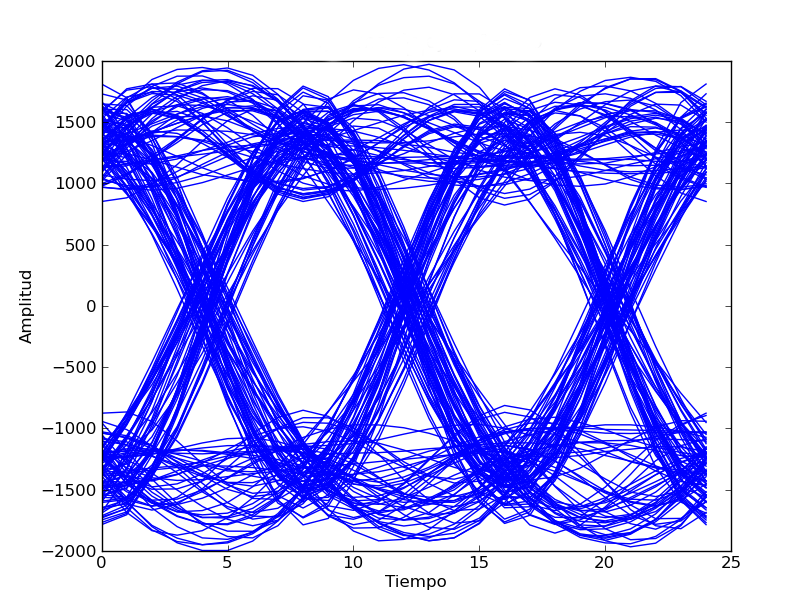
\includegraphics[scale=0.36]{figs/ojo35}}
  \subfloat[$\beta=0.50$]{\label{fig:eye50}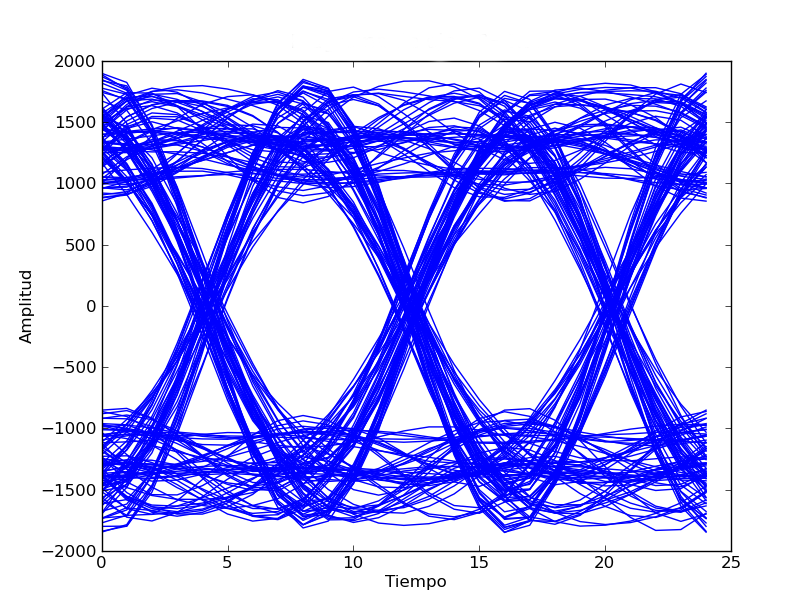
\includegraphics[scale=0.36]{figs/ojo50}}\\
  \subfloat[$\beta=0.75$]{\label{fig:eye75}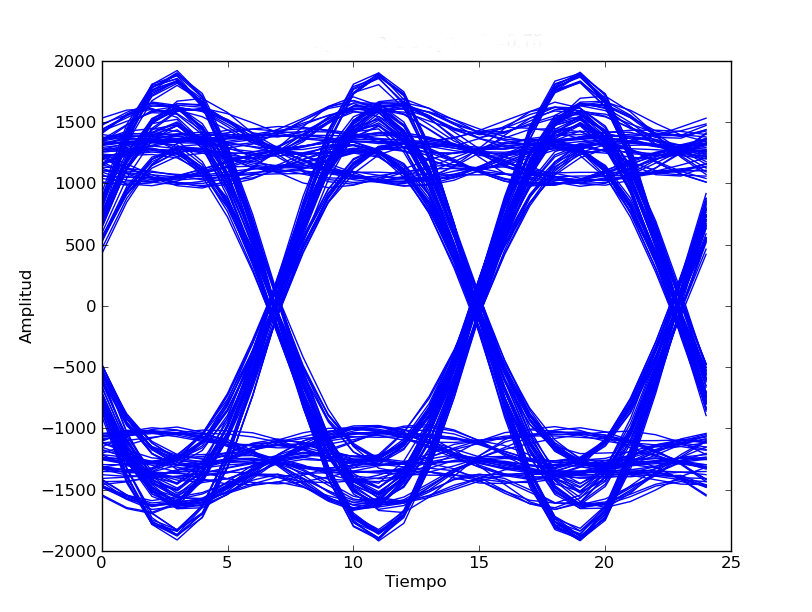
\includegraphics[scale=0.36]{figs/ojo75}}
  \vspace{0.3in}
  \caption{Se\~nales QPSK con filtrado de coseno elevado a diferentes valores de $\beta$.}
  \label{fig:rrcsignals}
\end{figure}

La figura \ref{fig:eye35} muestra que a menor $\beta$ la se\~nal se distorciona mas y esto causa mas
dificultades para detectar los s\'imbolos correctamente pero tambien resulta en un filtro mas rapido
sencillo de implementarse debido a que su respuesta al impulso es mas corta. La figura
\ref{fig:eye75} muestra menos distorcion en la se\~nal a consecuencia de un filtro mas complicado de
procesar eficientemente. El uso de mas ancho de banda tambien implica que se puede introducir mas
ruido en la etapa de captura de RF (front end) y por lo tanto es necesario considerar las
compensaciones entre el exceso de ancho de banda, la inmunidad contra el ruido, la complejidad de
la etapa de recuperacion del reloj de simbolos y la eficiencia de procesamiento por parte del CPU
\cite{lee}. El CPU Core 2 Duo que se utilizo fue suficiente para procesar filtros con $\beta$ de
0.75. Estos filtros son internamente implementados con una mezcla de lenguaje C y ensamblador utilizando
instrucciones como SSE (\emph{streaming SIMD extensions}) para incrementar la velocidad y eficiencia
de procesamiento.

El programa que genera el diagrama de ojo apartir de un archivo con muestras del USRP se muestra en
el listado \ref{ex:eyeprog}.
%FIXME: Explicar la funcion get_traces.
\begin{lstlisting}[float, label=ex:eyeprog, caption={Programa que genera el diagrama de ojo a partir
de muestras tomadas del USRP.}, breaklines=true]

import pylab as p
import struct
import scipy

samp_per_sym = 8
hfile = '/home/haysoos/Documents/Tesis/usrp_capture/target.dat'

def get_traces(d, num_traces, samp_per_sym):
    traces = []
    trace_len = samp_per_sym * 3
    for i in range(num_traces):
        start_ind = (samp_per_sym / 2) - 1 + (i + 3) * trace_len
        traces.append(d[start_ind:start_ind + trace_len + 1])
    return traces
    
 iq = scipy.fromfile(hfile, dtype = scipy.complex64)

ichan = [c.real for c in iq]

traces = get_traces(ichan, 200, samp_per_sym)
p.figure()
p.hold(True)
for tr in traces:
    p.plot(tr, 'b-')

p.title('Diagrama de ojo   ' + r'$\beta=0.75$')
p.xlabel('Tiempo')
p.ylabel('Amplitud')

p.show()
\end{lstlisting}

Una observaci\'on interesante es que los valores de tipo \emph{float} en Python equivalen al tipo
\emph{double} en C el cual puede variar dependiendo el CPU que se este utilizando pero en casos
tipicos la presicion es de 64 bits: 1 bit para el signo, 11 para el exponente y 52 para la mantisa.
\cite{python} El USRP configurado con el \emph{source} o \emph{sink} que utiliza el prefijo ``c''
utiliza la constante \verb|gr_complex| el cual equivale en lenguaje C a \emph{float}. Este tipo de
dato es de 32 bits: 1 bit para el signo, 8 bits para el exponente y 23 bits para la mantisa. Python
por default no tiene soporte para representar el tipo \emph{float} de C lo cual introduce errores en la
representacion de las muestras del USRP. La libreria \emph{Numpy} y \emph{Scipy} de Python encapsula
varias representaciones de numeros flotantes \cite{scipy} lo cual es necesario utilizar la correcta
cuando se trabaja con muestras que genera el USRP de manera independiente de los programas de
\emph{GNURadio}. Cada muestra compleja que transmite o recive el USRP es representado por dos
numeros flotantes de 32 bits por lo que es necesario utilizar el tipo de dato \emph{complex64} como
se muestra en el listado \ref{ex:eyeprog}.
%Constelacion observada
%==========================================================================
\section{Constelaci\'on observada}

%TODO: Incluir ambas imagenes de la constelacion para ilustrar los problemas que se tuvieron.
% Explicar el uso de QT (breve) para el desarrollo de interfazes de usuario y los 4 sinks que
% proporciona GR_QT (freq display, waterfall, time domain, constellation). Explicar como se
% transmitio la informacion aleatoria y el archivo fijo. Tambien explicar las modificaciones que se
% hisieron a benchmark_tx y rx para lograr la transmision correcta.
